\documentclass[a4paper,conference]{IEEEtran}
\usepackage[T1]{fontenc}
\usepackage{amsmath,amssymb,booktabs,array,graphicx}
\usepackage{tikz}
\usetikzlibrary{arrows.meta,positioning,calc}
\usepackage[hidelinks]{hyperref}
\usepackage{url}
\usepackage{pdfpages}
\definecolor{ink}{HTML}{19334A}
\definecolor{bluewash}{HTML}{EAF1F7}
\definecolor{greenwash}{HTML}{EAF4EE}
\definecolor{amberwash}{HTML}{FBF1DD}
\setlength{\tabcolsep}{4pt}
\title{TRAC-Engage: Track-Aware Multi-Agent Coordination for Continuous Video Engagement Estimation}
\author{\IEEEauthorblockN{Research Architecture Proposal}
\IEEEauthorblockA{Revised literature review and research implementation\\14 October 2026}}
\begin{document}
\maketitle
\begin{abstract}
Continuous engagement estimation requires more than classifying isolated face images: a system must localize people, preserve identities, model behavior over time, and recognize insufficient evidence. We review deep-learning approaches spanning convolutional recurrent networks, temporal convolutions, video transformers, multimodal attention, and agent-based inference. We propose TRAC-Engage, a video-first framework that produces persistent person bounding boxes and time-indexed engagement scores without requiring physiological sensors. Stateful specialist agents execute visual, temporal, and optional multimodal analyses; a learned coordinator allocates computation across people. The candidate contribution is track-conditioned, freshness-constrained evidence acquisition: specialist calls are selected by predicted reduction in engagement error, subject to latency and per-person refresh constraints, while a verifier prevents stale or identity-mismatched evidence from becoming a current score. Audio and physiological agents extend the architecture without replacing its visual core. We specify learning objectives, a streaming contract, ablations, and evaluation needed to establish an accuracy--latency benefit. This is a research architecture proposal; no unperformed experiments or measured superiority are reported.
\end{abstract}
\begin{IEEEkeywords}
engagement estimation, video understanding, multi-agent systems, adaptive inference, tracking, multimodal fusion
\end{IEEEkeywords}

\section{Introduction and Problem Definition}
The objective is to accept a recorded video or live stream and continuously return, for every observable person, a bounding box, persistent track identifier, engagement estimate, and evidence status. No Meridian session, task log, wearable, or manual sensor configuration is required for the video-only path. ``General'' describes an extensible system across learning, meetings, and human--computer interaction, not a claim that one training set yields universal psychological inference.

For frame $I_t$, the output is
\begin{equation}
\mathcal{O}_t=\{(k,b_{kt},s_{k\tau},\tau,c_{k\tau},v_{k\tau})\}_{k\in\mathcal{K}_t},
\end{equation}
where $k$ identifies a track, $b$ is its current box, $s\in[0,100]$ is an engagement index computed at $\tau\le t$, $c$ summarizes predictive confidence, and $v$ indicates valid, warming up, stale, or insufficient evidence. Detection confidence is separate. Boxes may update every frame while scores update once per second; displaying the last estimate does not create a new frame-level measurement.

The target is observable task/conversation engagement under a declared annotation protocol. Video cannot uniquely reveal internal attention: looking away can indicate thinking, and eye contact can occur without understanding. Without contextual information, the system estimates externally expressed involvement, with abstention outside validated conditions. It must not reinterpret happiness, stress, or task success as engagement labels.

\section{Research Review: From Clip Models to Agentic Inference}
\subsection{Scope and Comparison Criteria}
This targeted review covers primary engagement papers and enabling video, tracking, fusion, and agent research available through 14 October 2026. Searches combined engagement estimation with temporal CNN, transformer, multimodal fusion, tracking, adaptive inference, and multi-agent terms. We compare representation, temporal support, output granularity, domain transfer, and computation. This is a focused narrative review, not an exhaustive systematic review. Table~\ref{tab:review} summarizes design consequences. Published accuracies are not ranked across incompatible label definitions and splits.

\subsection{CNN--RNN, 3D CNN, and Temporal Convolution}
DAiSEE established a four-level engagement benchmark alongside other affective annotations and investigated image/video baselines, including 3D convolution and recurrent temporal modeling \cite{daisee}. A frame CNN learns appearance but misses persistence and transitions. CNN--LSTM/GRU adds sequence memory; 3D CNN learns short spatiotemporal patterns jointly, with a larger clip-processing burden. Neither inherently supplies persistent person identities or calibrated streaming outputs.

Abedi and Khan's ResNet--TCN combines learned frame features with temporal convolutions for engagement classification \cite{tcn}. Dilated causal convolutions are attractive for bounded-memory inference; converting a clip classifier to a streaming estimator still requires explicit history, warm-up, and label alignment. We choose this family as the inexpensive always-on visual path, and retain CNN--GRU and 3D CNN as controls rather than presuming transformers always win.

\subsection{Video Transformers and Representation Learning}
CavT uses class attention and representative sampling to handle engagement videos of different lengths \cite{cavt}. It motivates learned aggregation instead of frame averaging, but whole-video sampling cannot enter online inference if it accesses future frames. EngageNet compares temporal models using gaze, head pose, facial actions, and learned facial representations \cite{engagenet}. Its feature-combination and cross-dataset experiments show why adding features and achieving within-dataset accuracy do not establish generality.

VideoMAE supplies self-supervised spatiotemporal pretraining \cite{videomae}. It is a video-representation framework, not an engagement detector: an engagement head must be trained on engagement labels. We use a pretrained VideoMAE encoder as an on-demand motion expert over a trailing crop sequence, not an expensive mandatory model for every person at every frame. Attention within that already-observed clip is permitted; no future relative to the output time is available.

\subsection{Interaction, Multimodal Fusion, and Domain Transfer}
DAPA combines audiovisual features, domain prompts, and parallel attention between conversational partners \cite{dapa}. Its backward recurrent states use future context, so its reported offline setting must be separated from a causal streaming adaptation. It also shows why conversational engagement depends on interaction rather than an isolated face. Partner association will be optional and based on known interaction context, not proximity alone.

MulT provides cross-modal attention for unaligned sequences \cite{mult}, while bottleneck fusion restricts exchange through a small latent set \cite{mbt}. Both are architectural foundations, not engagement-specific proof. We adopt intermediate fusion because early concatenation is brittle when streams disappear, while pure late voting discards interactions. Multiple visual crops remain one sensing modality; audio or physiology makes the system genuinely multimodal.

CMOSE supplies ordered engagement labels with visual, acoustic and transcript representations, and introduces MocoRank to address within-class variation and ordinal structure \cite{cmose}. It is particularly useful for a reproducible CPU pilot because its authors release precomputed features publicly. We use those features to test the fusion/ordinal core, not to claim replication of MocoRank or validation of our proposed tracking and scheduling stack. Transcript availability is an experimental extension, not a requirement of the video-only architecture.

\subsection{What Multi-Agent Research Already Provides}
\textbf{Updated engagement-specific prior art.} CORE-Net combines skeleton, behaviour and facial representations with contextual attention and an ordinal objective on COLER \cite{core}. Safa et al. address ordinal engagement and imbalance through supervised contrastive learning \cite{ordinaleng}. BCTR models ocular, head and trunk regions using temporal transformers \cite{bctr}. Therefore, ordinal supervision, region specialization and context fusion are \emph{not} claimed as our novelty.

MultiMediate'25 evaluates transfer across interaction domains and languages \cite{mm25}; its reported domain drops motivate independent transfer tests. The publicly posted MultiMediate'26 specification adds distinct task/social targets in PInSoRo \cite{mm26}. Its repository is available before the listed November proceedings date; we cite the current specification, not a future completed evaluation. Categorical task engagement and continuous conversational involvement cannot be merged by rescaling labels alone.

Sun and Feng's Engagement Dynamics Forecaster includes interacting recurrent agents and uncertainty regularization \cite{edf}. Thus, we do not claim to introduce multi-agent engagement prediction. The relevant distinction is between interacting latent states and agents that decide whether to acquire additional evidence under an execution budget. LVAgent coordinates multimodal language-model agents for long-video question answering \cite{lvagent}; iterative deliberation for that task differs from numerical engagement estimation with per-person deadlines. AdaFrame already learns adaptive observation selection for efficient video recognition \cite{adaframe}. Adaptive computation is also prior art.

\textbf{Gap and hypothesis.} These mechanisms do not, by themselves, establish the benefit of joint identity-aware evidence expiry, per-track service constraints, and cost-sensitive specialist acquisition for continuous engagement. Our hypothesis is a better engagement-error versus latency/coverage frontier than fixed fusion or uncertainty-only scheduling. This is a testable contribution, not a verified first-in-literature claim.

\begin{table*}[t]
\caption{Framework-level review and implications for streaming inference. These are methodological comparisons, not a cross-paper accuracy leaderboard.}
\label{tab:review}\centering\footnotesize
\begin{tabular}{p{.19\textwidth}p{.35\textwidth}p{.39\textwidth}}
\toprule
Framework family & Mechanism / relevant evidence & Limitation for this goal and adopted design choice\\
\midrule
DAiSEE \cite{daisee}; ResNet--TCN \cite{tcn} & Appearance encoders followed by recurrent, 3D, or temporal convolutional inference. & Clip labels are not dense trajectories. Use a causal low-cost visual branch and evaluate continuity separately.\\
CavT \cite{cavt}; EngageNet \cite{engagenet} & Class attention, representative sampling, facial descriptors, and temporal transformers. & Offline sampling and dataset cues can leak into streaming claims. Use trailing windows and person-disjoint tests.\\
VideoMAE \cite{videomae} & Masked-video pretraining for transferable spatiotemporal representations. & Not pretrained to measure engagement. Fine-tune a specialist and invoke it selectively.\\
DAPA \cite{dapa} & Domain conditioning and partner-aware audiovisual temporal attention. & Future-informed states differ from online inference. Compare offline and strictly causal variants.\\
MulT \cite{mult}; bottleneck fusion \cite{mbt} & Cross-modal temporal interaction and restricted latent exchange. & Fusion alone does not schedule tools or protect identity. Add masked evidence contracts and coordination.\\
EDF \cite{edf}; LVAgent \cite{lvagent}; AdaFrame \cite{adaframe} & Agent interaction, collaborative video reasoning, and adaptive computation. & These establish prior art. Test per-track freshness and budget allocation against the relevant design principles.\\
\bottomrule
\end{tabular}
\end{table*}

\section{TRAC-Engage: Detailed Architecture}
\subsection{Detection, Association, and Track Memory}
The tracking agent uses an RT-DETR person detector \cite{rtdetr} and ByteTrack association \cite{bytetrack}. Detection initializes or corrects boxes; tracking propagates identities between detections. Face crops are associated with their enclosing person and temporal trajectory. Tight webcam framing, partial bodies, and small faces require a face-aware fallback and explicit validation; absence of a person box is not low engagement.

Each track owns a timestamped crop buffer, feature cache, quality history, and identity generation number. Suspected identity swaps, scene cuts, and uncertain re-entry invalidate cached engagement evidence. A new identity warms up instead of inheriting another person's score. Pseudonymous track IDs are not biometric recognition. Detection runs at an initial 5 Hz target with association between detections; recovery can request immediate re-detection. All rates are proposed settings to be profiled.

\begin{figure*}[t]
\centering
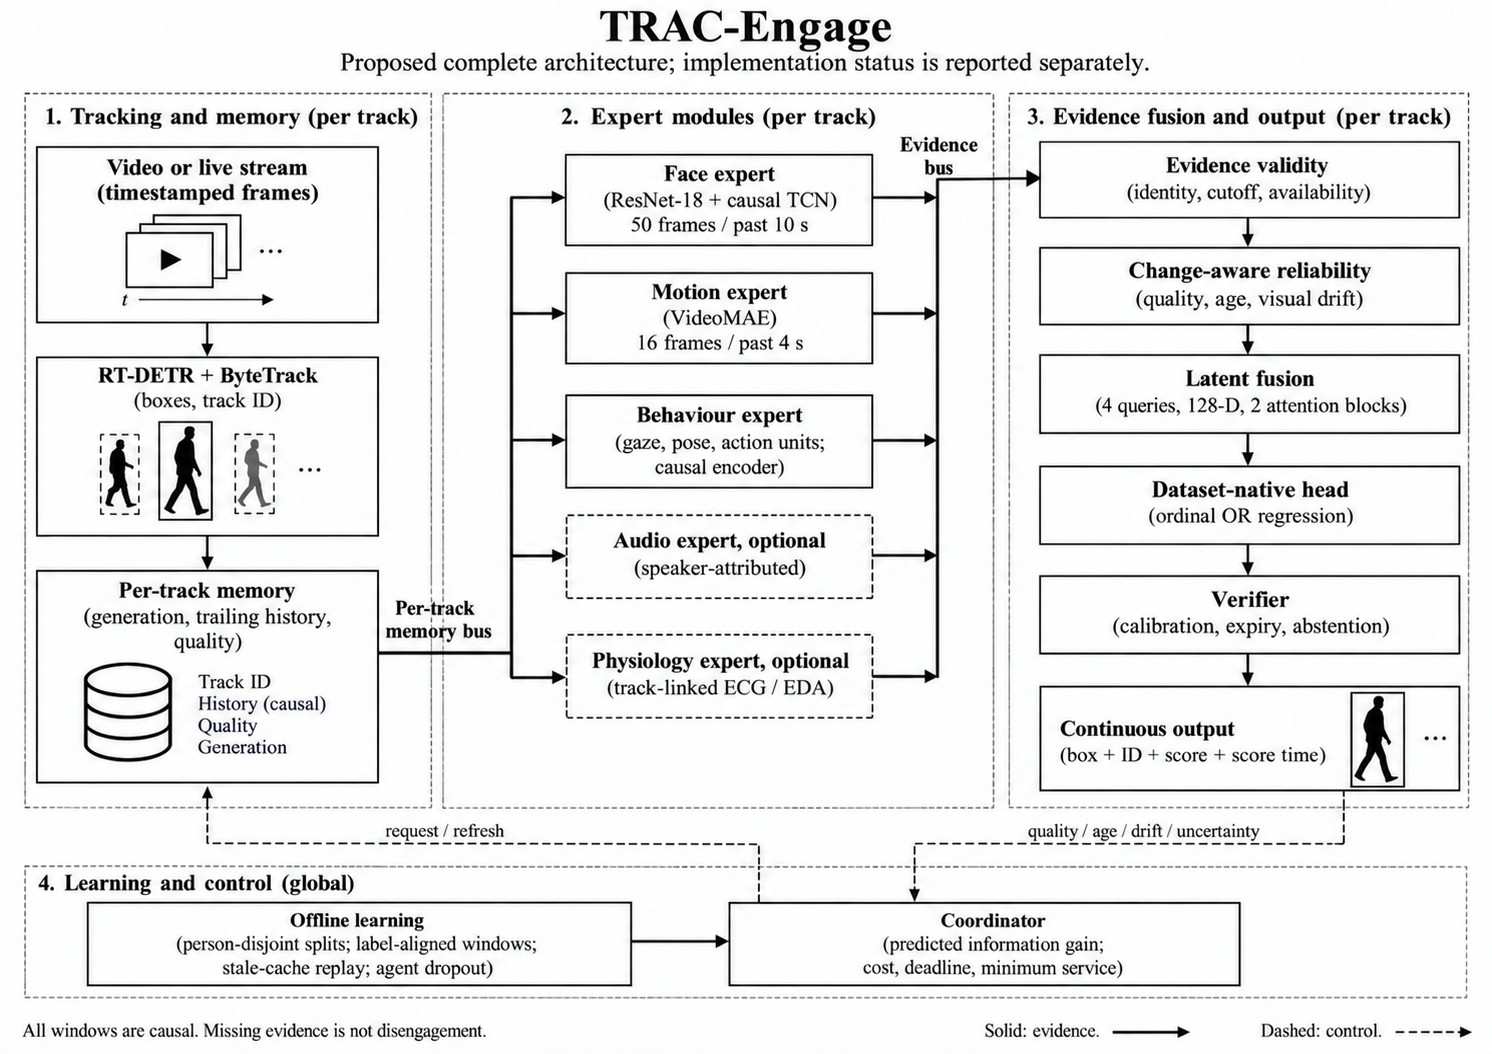
\includegraphics[width=.93\textwidth]{trac-engage-v2-architecture.png}%
\caption{Proposed complete TRAC-Engage pipeline. Evidence passes through validity, change-aware reliability, fusion, a dataset-native head and verification, in that order. Metadata includes current boxes and track generation. Dashed paths are control. Optional audio and physiology require independent synchronized inputs linked to the track; they are not inferred from video. A full-size A4 landscape version is appended. This illustration does not imply that every branch has been implemented or validated.}
\label{fig:arch}
\end{figure*}

\subsection{Specialist Agents and Deep Encoders}
\textbf{Face agent:} 224$\times$224 face crops sampled at 5 fps over the preceding 10 s enter a pretrained ResNet-18 and a causal TCN. The research implementation uses one kernel-3 convolution per residual block with dilations 1, 2, and 4, channel-wise LayerNorm and a mean over all observed temporal outputs. The last TCN position alone sees only 15 samples; history pooling is necessary to cover all 50 input frames. Landmark alignment is a planned upgrade to the current unique-face crop baseline. The branch emits a 128-dimensional token. Auxiliary heads are a planned training ablation; face quality is separate from engagement.

\textbf{Motion agent:} on request, VideoMAE-base processes 16 person-crop frames from the past 4 s and projects its embedding to 128 dimensions. It supplies motion context when facial interpretation is ambiguous, without treating every movement as disengagement. Initial training freezes most pretrained weights, then unfreezes upper blocks if participant-disjoint validation supports it.

\textbf{Behavior agent:} OpenFace-derived facial actions, coarse gaze, and head-pose trajectories \cite{openface} enter a small causal temporal encoder. It supplies an interpretable complementary representation, not a gaze-to-engagement rule. Webcam gaze is not precise eye tracking. Face and behavior agents share correlated evidence; fusion must not treat their agreement as independent confirmation.

\textbf{Optional agents:} audio prosody and turn statistics require speaker attribution and a temporal encoder; unassigned room sound is masked. ECG and EDA use separate temporal encoders and validity masks. A wearable must be explicitly linked to a track, never assigned by visual proximity. Agents cannot manufacture unavailable observations. Visual-only input is a multi-view model; audiovisual or physiological input activates multimodal fusion.

\subsection{Why These Are Agents, Not Renamed Layers}
Each specialist maintains per-track state, receives requests, chooses permitted operations such as feature refresh, valid-crop re-extraction, or returning unavailable, and publishes typed evidence. The tracking agent can recover association; the verifier rejects evidence and requests one bounded retry. The coordinator learns acquisition choices under a shared budget. Neural branches alone are experts, not agents; memory, actions, and feedback constitute the agentic execution layer.

This is a centralized cooperative multi-agent workflow, not a claim that all components are autonomous LLMs or that multi-agent reinforcement learning has been implemented. No language-model debate occurs on the frame-critical path. An optional reporting LLM may explain recorded decisions afterward, but cannot alter scores or substitute a narrative for missing evidence.

\subsection{Candidate Novelty: Track-Conditioned Evidence Acquisition}
For track $k$ and optional specialist $m$, the coordinator observes state $z_{kt}$: quality, evidence age, cached prediction disagreement, association confidence, and queue state. It predicts supervised-loss reduction $\widehat{\Delta\ell}_{km}$ from refreshing that specialist. Calls solve a constrained allocation:
\begin{align}
\max_{a_{km}\in\{0,1\}}\quad &\sum_{k,m}a_{km}(\widehat{\Delta\ell}_{km}-\lambda c_{km}),\label{eq:policy}\\
\text{s.t.}\quad &\sum_{k,m}a_{km}c_{km}\le B_t,\nonumber
\end{align}
where $c$ is profiled incremental cost and $B_t$ the budget remaining after tracking and base inference. Calls must finish before the output deadline. Costs include batch/queue effects; agents are not free parallel workers. A greedy approximation is acceptable if its regret against the small-instance optimum is measured.

The contribution is not Eq.~\ref{eq:policy} alone. It couples acquisition to \emph{identity generation, evidence expiry, and a minimum base-service rate per visible person}. Identity changes cancel outstanding requests; expired messages cannot count as fresh evidence. Base service is reserved before optional calls so uncertain people cannot consume the entire budget. If base service itself is infeasible, round-robin allocation explicitly reports stale/insufficient evidence rather than silently excluding quiet people. Service constraints are not demographic fairness guarantees.

For utility learning, all specialists run on training-development examples to construct losses with and without refreshed results, using out-of-fold base predictions. At deployment the coordinator sees only pre-call state, never the label or unobserved expert output. Training-sequence rollouts expose stale-cache states for subsequent fitting. This supervised value-of-information policy is simpler to audit than unrestricted online reinforcement learning. Correlated gains and inaccurate cost estimates remain testable failure modes.

\subsection{Masked Fusion and Score Semantics}
\textbf{Additional candidate novelty: change-aware cache replay.} A token can be young yet obsolete after a rapid behavioural change. Let $u_{kt}$ be the normalized cheap visual embedding and $t_m$ the last expert acquisition time. Define visual drift $\delta_{km}=\max(0,1-u_{kt}^{\top}u_{kt_m})$. Drift is an observable appearance change, \emph{not} an engagement transition label. We test whether penalizing drift in reliability and supplying it to the pre-call coordinator reduces transition delay at fixed cost. Occlusion or camera motion can also raise drift; quality and tracking validity must be checked first.

Accepted tokens contain features $h_{km}$, quality $q_{km}$, age $d_{km}$, and identity/support metadata. Reliability is
\begin{equation}
r_{km}=v_{km}q_{km}\exp(-d_{km}/\tau_m-\beta_m\delta_{km}),
\end{equation}
where $v=0$ for wrong identity, expired, absent, or invalid evidence. Four latent queries aggregate 128-D tokens through two four-head attention blocks, with $\log(r+\epsilon)$ bias and hard masking when $v=0$. Each specialist contributes a fixed token count. Early concatenation and probability-level late fusion remain baselines.

To make this mechanism learnable under realistic caches, training will replay delayed expert tokens from \emph{earlier windows of the same track and generation}, retaining their true support intervals. All-expert training-only rollouts supply counterfactual loss differences. No random token from another participant is a valid stale observation. We compare age-only reliability ($\beta=0$), drift-aware reliability, and both with replay. The implemented reliability rule is deterministic; its benefit and the learned utility policy remain unvalidated. This combined mechanism is a research hypothesis, not a first-in-literature assertion.

For four-level datasets, an ordered-threshold head predicts $o_j=P(y>j)$ for $j=0,1,2$, giving $p=(1-o_0,o_0-o_1,o_1-o_2,o_2)$ and
\begin{equation}
s=\frac{100}{3}\sum_{j=0}^{3}jp_j.
\end{equation}
This is an ordinal expectation, not a literal percentage of attention. Continuous-annotation datasets use a separate sigmoid regression head with CCC and MAE losses; scales are not silently pooled. Confidence is calibrated on held-out people \cite{guo}. The verifier applies validation-set thresholds for usable evidence and rejection, evaluated with risk--coverage curves \cite{selective}. Calibration is not guaranteed under unseen domains.

Ordered cutpoints are implemented as $\theta_j=\theta_0+\sum_{i=1}^{j}\operatorname{softplus}(g_i)$ with $o_j=\sigma(a(h)-\theta_j)$. Thus probabilities remain non-negative by construction, drawing on rank-consistent ordinal modelling \cite{coral}. This is an established modelling choice, not a separate novelty claim. All-missing inputs return an unusable status, never an apparently meaningful zero score.

\section{Continuous Workflow and Multimodal Extension}
Frames are decoded once; tracking and extraction share caches and batch crops across people. Each one-second decision uses only data available by its cutoff. The first ten seconds are warm-up; shorter-history operation requires separate validation. Annotated video preserves presentation timestamps, attaches score time, and marks unavailable scores ``--''. A lost track is not disengaged. Figure~\ref{fig:output} illustrates the output contract.

\begin{figure}[t]
\centering
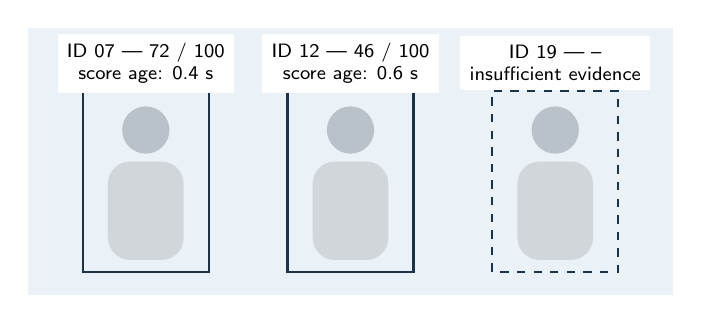
\begin{tikzpicture}[x=1cm,y=1cm,font=\sffamily\scriptsize]
\fill[bluewash] (0,0) rectangle (8.2,3.4);
\foreach \x in {1.5,4.1,6.7} {\fill[ink!30] (\x,2.1) circle (.3);\fill[ink!20,rounded corners=8pt] (\x-.48,.45) rectangle (\x+.48,1.7);}
\draw[ink,thick] (.7,.3) rectangle (2.3,2.6);
\draw[ink,thick] (3.3,.3) rectangle (4.9,2.6);
\draw[ink,dashed,thick] (5.9,.3) rectangle (7.5,2.6);
\node[fill=white,align=center] at (1.5,2.95) {ID 07 | 72 / 100\\score age: 0.4 s};
\node[fill=white,align=center] at (4.1,2.95) {ID 12 | 46 / 100\\score age: 0.6 s};
\node[fill=white,align=center] at (6.7,2.95) {ID 19 | --\\insufficient evidence};
\end{tikzpicture}
\caption{Illustrative output, not an experiment or actual inference screenshot. Boxes locate people; scores use temporal evidence. Numbers are synthetic examples. Uncertain evidence produces an explicit status rather than a low engagement score.}
\label{fig:output}
\end{figure}

The initial target is one 720p stream with 1--8 visible people, one score update/s, and p95 post-window processing below 500 ms on a declared GPU workstation. These are profiling targets, not measured capabilities. Score expiry starts at 2 s; token expiry is specialist-specific. Event-time latency, queue delay, warm-up, and rendering rate are reported separately. Bounded queues discard obsolete optional jobs before delaying tracking; original video need not be dropped with analysis work.

Meridian is one later source of linked multimodal recordings, not an architectural dependency. ECG, EDA, and optional task events enter the evidence contract after synchronization, engagement-specific annotation, and participant-to-track linkage. Autonomic fusion has precedent in personalized engagement research \cite{rudovic}, not proof of transfer across populations. Missing-modality training retains a separately tested visual-only path. Pulse oximetry, thermal imaging, and every other connected device are not required by default.

\section{Training, Evaluation, and Falsifiable Claims}
\subsection{Training and Label Granularity}
We train visual experts first, then fusion with modality/agent dropout, then coordination, and recalibrate under the deployed policy because selective execution changes the prediction distribution. Ordinal heads minimize cumulative binary cross-entropy; continuous heads minimize weighted $1-\mathrm{CCC}$ and MAE. Auxiliary expert losses support useful individual branches. Loss weights and unfreezing schedules are selected inside training/validation folds.

DAiSEE and EngageNet supply clip-level starting points, not ground truth for every frame. Loss applies to annotated support intervals; clip labels are not duplicated as independent dense labels. Conversational datasets discussed in DAPA provide complementary continuous-label evaluation. A consented, densely annotated multi-person set is still needed to validate association and transitions in the target setting. Independent annotators score involvement, not presumed emotion; inter-rater agreement and disagreement are reported.

People, sessions, and overlapping windows remain within one split. Subject-disjoint training, model-selection, calibration, and locked test partitions are supplemented by held-out task/site/device conditions. Dataset-native heads avoid false equivalence between attentional and conversational labels. Zero-shot, calibrated, and fine-tuned transfer are reported separately. Engagement test people cannot enter adaptation or coordinator training.

\subsection{Baselines and Necessary Ablations}
The comparison ladder is frame CNN, CNN--GRU, ResNet--TCN, 3D CNN, CavT/VideoMAE engagement fine-tuning, fixed early/late/bottleneck fusion, and coordinated experts. Offline DAPA and a causal counterpart are separate references. To isolate agency, decisive baselines reuse \emph{identical} experts with always-on, uniform-periodic, random, and uncertainty-only execution at matched measured budgets. An EDF-style recurrent-agent baseline tests scheduling beyond latent agent interaction.

Remove utility learning, identity invalidation, expiry, and minimum service individually. Exclude behavior, audio, or physiology to measure incremental utility. Compare the same coordinator in a single process: scheduling benefit does not establish that distributed deployment is necessary. At least three seeds and participant-cluster bootstrap intervals are required.

The new factorial ablation crosses age-only versus age-and-drift reliability with fresh-only versus stale-cache-replay training. Hold encoders, folds, compute and coverage constant. Measure transition delay and stale-score duration in addition to ordinal MAE. A second, deferred direction is multimodal-teacher distillation into the video student on consented paired data. It requires teacher/student mask-aware losses and video-only testing; neither distillation nor extra modalities constitute novelty by themselves. We do not add an LLM voting loop without an accuracy--latency justification.

\begin{table}[t]
\caption{Evaluation measures the entire output contract.}\centering\footnotesize
\begin{tabular}{p{.24\columnwidth}p{.68\columnwidth}}
\toprule
Dimension & Required measurements\\
\midrule
Engagement & Macro-F1, balanced accuracy, ordinal MAE; CCC/MAE for continuous labels.\\
Localization & Box AP/IoU, track IDF1, identity switches, missed-person coverage.\\
Reliability & NLL/Brier, calibration plots, risk--coverage, error at equal coverage.\\
Continuity & Score age, transition delay, stale-score exposure, wrong-person score duration.\\
Efficiency & p50/p95 latency, GPU time, calls, queue misses, memory, throughput versus people.\\
Service equity & Refresh/abstention per track and capture condition; disaggregated errors where supported.\\
\bottomrule
\end{tabular}
\end{table}

Fault tests include occlusion, small crops, camera cuts, crossing people, re-entry, frame loss, missing audio, sensor delay, and increasing person count. A scheduler must not improve accuracy simply by refusing difficult people: report all visible-person time, abstention, and matched-coverage error. The primary claim succeeds only if coordination improves the accuracy--latency frontier while limiting stale and misassigned scores. If threshold scheduling matches it, or overhead removes the gains, multi-agent novelty is not supported.

\section{Implementation Status and Completed Engineering Checks}
We implemented an isolated PyTorch research package with causal temporal experts, reliability-masked latent fusion, ordered cutpoints, manifest/split validation, AdamW training, validation-only model selection, temperature calibration and held-out metrics. The development video path uses a unique frontal Haar face crop and frozen ImageNet ResNet-18, not the proposed RT-DETR/ByteTrack multi-person pipeline. The learned coordinator, full specialist extractors and stale-cache replay remain unimplemented. A greedy utility/cost helper is a scheduling baseline, not a trained policy.

A CPU software test trained on generated arrays: 64 training and 24 validation examples, four artificial classes, 20 time steps, eight input features and width 32. Across 12 epochs, cumulative training loss decreased from 0.3472 to 0.2183. Separate synthetic calibration and test partitions exercised checkpoint loading and metrics. These are \emph{engineering checks, not engagement experiments}; they do not establish human-data accuracy, architectural benefit, generalization or real-time throughput. The inference entry point refuses synthetic checkpoints. Tests cover causality, masking, ordered probabilities, identity/time validity, missing data, gradients, budget limits and participant leakage.

Official dataset access was reviewed on 14 October 2026. DAiSEE requires a research-use request and lists an approximately 15-GB compressed corpus \cite{daiseeaccess}. DIPSER/DIPSEER offers engagement annotations under CC BY 4.0, but the complete release is approximately 668 GB \cite{dipser}; a bounded labelled subset was not successfully retrieved. We instead downloaded the CMOSE authors' public feature release under CC BY-SA 4.0 and verified its published SHA-256 hashes \cite{cmose}. The Windows environment is CPU-only PyTorch; Intel Arc acceleration was not configured. No deployment was performed.

\subsection{Public-Data Pilot: Protocol and Scope}
The two downloaded JSON files contain 12,197 labelled records; 295 have empty I3D embeddings and are excluded with logged reasons, leaving 11,902 clips. Inputs are one 1024-D I3D vector, one 768-D BERT vector and six acoustic summaries per clip. Label agreement is not an input. Training-only standardization is applied per channel, clipping standardized values to $[-10,10]$. Each branch has one temporal token, so this experiment does \emph{not} validate temporal convolutions, dense scores, tracking, quality estimation or stale-cache novelty.

We replace the release's clip-level split with a predetermined whole-session partition: sessions 1, 5, 6, 7, 14 and 18 train (8,806 clips), session 15 validates (709), session 16 calibrates (734), and session 10 is locked for testing (1,653). These are session-disjoint splits. Released person IDs are session-scoped; cross-session biological identity cannot be verified, so globally subject-disjoint evaluation is not claimed. Only one session is held out for testing, and the calibration partition contains only one lowest-engagement example, limiting tail calibration and generalization conclusions.

The bounded pilot compares visual-only mean fusion, visual/acoustic/text mean fusion, and the same multimodal inputs with latent attention. All use width 32 and the same ordinal head, AdamW, batch 128, gradient clipping and 0.2 branch dropout. Learning rates $3\times10^{-4}$ and $10^{-3}$ are compared on validation MAE using seed 17; selected rates are locked before seeds 31 and 53 and before test evaluation. Training is capped at ten epochs with patience four. Positive temperature scaling uses only session 16. This is a feature-level ablation, not a matched-budget agentic study or a comparison with the original CMOSE leaderboard.

\subsection{Completed Pilot Results and Negative Findings}
All 12 training runs completed; nine selected-model evaluations cover three configurations and three seeds. Validation selected $10^{-3}$ for each configuration. Table~\ref{tab:pilot} reports test results after calibration, with seed standard deviation rather than a confidence interval. The majority class is chosen from training counts, not test labels. All retained feature examples are usable; this 100\% feature coverage is conditional on the 295 exclusions and does not measure coverage of people in video.

\begin{table*}[t]
\centering\small
\caption{Actual CMOSE custom session-held-out feature pilot, 1,653 test clips. Mean $\pm$ seed SD over seeds 17, 31 and 53. Accuracy, macro-F1 and balanced accuracy are percentages; MAE is in native 0--3 class units. These results do not validate the proposed multi-agent architecture.}
\label{tab:pilot}
\begin{tabular}{lrrrrr}
\toprule
Configuration & Accuracy & Macro-F1 & Balanced acc. & Calibrated MAE & Uncalibrated MAE\\
\midrule
Training-majority constant & 62.13 & 19.16 & 25.00 & 0.415 & 0.415\\
Visual mean & $40.53\pm2.88$ & $24.76\pm1.85$ & $33.83\pm0.63$ & $0.691\pm0.032$ & $0.500\pm0.009$\\
Multimodal mean & $47.45\pm9.26$ & $25.36\pm4.20$ & $33.60\pm1.89$ & $0.647\pm0.089$ & $0.477\pm0.007$\\
Multimodal latent & $41.80\pm15.31$ & $25.39\pm6.64$ & $34.29\pm2.74$ & $0.662\pm0.102$ & $0.464\pm0.008$\\
\bottomrule
\end{tabular}
\end{table*}

Learned models improve macro-F1 and balanced accuracy over the constant predictor, but all lose on overall accuracy and ordinal MAE. Multimodal latent attention does not consistently outperform simpler mean fusion. Its seed variation is substantial. Temperature scaling fitted for NLL on session 16 worsens expected-level MAE on session 10 for every configuration; calibration on one differently distributed session is not a reliability guarantee. The results support neither production use nor an empirical novelty claim.

Limited optimization, class imbalance, head specification and session shift are plausible, unproven contributors. Development-only studies must test head initialization, loss alignment and class-balanced learning with leave-one-session-out validation. Retuning on session 10 would invalidate its locked-test interpretation. Coordination, replay, tracking and live latency remain untested. Feature checkpoints cannot replace ResNet video weights.

\section{Limitations and Conclusion}
Internal engagement is not fully observable from video. Labels are contextual, cultures and disabilities affect expression, and physiology is confounded by activity and stress. Use requires consent, minimization, access control, and explicit uncertainty; scores are not grounds for grading, discipline, or diagnosis. Agent explanations are not causal evidence. Quantitative comparisons and prior-art review must be updated before submission.

TRAC-Engage combines tracking, temporal specialists and constrained acquisition, with optional audio and physiology. Its candidate contribution couples drift-aware freshness with same-track stale-cache replay. The implemented fusion core's CMOSE pilot exposes weak cross-session performance and calibration transfer, not superiority. Empirical novelty, full integration and study approvals remain future requirements.

\begin{thebibliography}{26}
\bibitem{daisee} A. Gupta, A. D'Cunha, K. Awasthi, and V. Balasubramanian, ``DAiSEE: Towards user engagement recognition in the wild,'' arXiv:1609.01885, 2016, revised 2022. \url{https://arxiv.org/abs/1609.01885}.
\bibitem{tcn} A. Abedi and S. S. Khan, ``Improving state-of-the-art in detecting student engagement with Resnet and TCN hybrid network,'' arXiv:2104.10122, 2021. \url{https://arxiv.org/abs/2104.10122}.
\bibitem{cavt} X. Ai, V. S. Sheng, C. Li, and Z. Cui, ``Class-attention video transformer for engagement intensity prediction,'' arXiv:2208.07216, 2022. \url{https://arxiv.org/abs/2208.07216}.
\bibitem{engagenet} M. Singh, X. Hoque, D. Zeng, Y. Wang, K. Ikeda, and A. Dhall, ``Do I have your attention: A large scale engagement prediction dataset and baselines,'' arXiv:2302.00431, 2023. \url{https://arxiv.org/abs/2302.00431}.
\bibitem{videomae} Z. Tong, Y. Song, J. Wang, and L. Wang, ``VideoMAE: Masked autoencoders are data-efficient learners for self-supervised video pre-training,'' in \emph{NeurIPS}, 2022. \url{https://arxiv.org/abs/2203.12602}.
\bibitem{dapa} Y. Yu et al., ``Generalizable engagement estimation in conversation via domain prompting and parallel attention,'' arXiv:2508.14448, 2025. \url{https://arxiv.org/abs/2508.14448}.
\bibitem{mult} Y.-H. H. Tsai et al., ``Multimodal transformer for unaligned multimodal language sequences,'' in \emph{ACL}, 2019, pp. 6558--6569. \url{https://aclanthology.org/P19-1656/}.
\bibitem{mbt} A. Nagrani et al., ``Attention bottlenecks for multimodal fusion,'' in \emph{NeurIPS}, 2021. \url{https://arxiv.org/abs/2107.00135}.
\bibitem{edf} M. Sun and S. Feng, ``Deep learning for student engagement analysis in educational psychology,'' \emph{Frontiers in Psychology}, vol. 17, art. 1764399, 2026, doi: \href{https://doi.org/10.3389/fpsyg.2026.1764399}{10.3389/fpsyg.2026.1764399}.
\bibitem{lvagent} B. Chen et al., ``LVAgent: Long video understanding by multi-round dynamical collaboration of MLLM agents,'' in \emph{ICCV}, 2025, pp. 20237--20246. \url{https://arxiv.org/abs/2503.10200}.
\bibitem{adaframe} Z. Wu, C. Xiong, C.-Y. Ma, R. Socher, and L. S. Davis, ``AdaFrame: Adaptive frame selection for fast video recognition,'' in \emph{CVPR}, 2019, pp. 1278--1287. \url{https://arxiv.org/abs/1811.12432}.
\bibitem{rtdetr} Y. Zhao et al., ``DETRs beat YOLOs on real-time object detection,'' in \emph{CVPR}, 2024, pp. 16965--16974. \url{https://arxiv.org/abs/2304.08069}.
\bibitem{bytetrack} Y. Zhang et al., ``ByteTrack: Multi-object tracking by associating every detection box,'' in \emph{ECCV}, 2022. \url{https://arxiv.org/abs/2110.06864}.
\bibitem{openface} T. Baltru\v{s}aitis, A. Zadeh, Y. C. Lim, and L.-P. Morency, ``OpenFace 2.0: Facial behavior analysis toolkit,'' in \emph{IEEE FG}, 2018, pp. 59--66, doi: \href{https://doi.org/10.1109/FG.2018.00019}{10.1109/FG.2018.00019}.
\bibitem{guo} C. Guo, G. Pleiss, Y. Sun, and K. Q. Weinberger, ``On calibration of modern neural networks,'' in \emph{ICML}, 2017, pp. 1321--1330. \url{https://proceedings.mlr.press/v70/guo17a.html}.
\bibitem{selective} Y. Geifman and R. El-Yaniv, ``SelectiveNet: A deep neural network with an integrated reject option,'' in \emph{ICML}, 2019, pp. 2151--2159. \url{https://proceedings.mlr.press/v97/geifman19a.html}.
\bibitem{rudovic} O. Rudovic, J. Lee, M. Dai, B. Schuller, and R. W. Picard, ``Personalized machine learning for robot perception of affect and engagement in autism therapy,'' \emph{Science Robotics}, 2018. \url{https://arxiv.org/abs/1802.01186}.
\bibitem{core} N. Tran, D. Ly, P. Ta, H. Nguyen, and H. D. Nguyen, ``Ordinal-aware multimodal engagement recognition for collaborative learning,'' in \emph{WACV}, 2026, pp. 2424--2433. \url{https://doi.org/10.1109/WACV61042.2026.00239}.
\bibitem{ordinaleng} S. Safa, A. Abedi, and S. S. Khan, ``Supervised contrastive learning for ordinal engagement measurement,'' arXiv:2505.20676, 2025. \url{https://arxiv.org/abs/2505.20676}.
\bibitem{bctr} Y. Bei, S. Guo, K. Gao, and Z. Feng, ``Behavior capture guided engagement recognition,'' \emph{Pattern Recognition}, vol. 164, art. 111534, 2025. \url{https://doi.org/10.1016/j.patcog.2025.111534}.
\bibitem{mm25} D. S. Withanage Don et al., ``MultiMediate '25: Cross-cultural multi-domain engagement estimation,'' in \emph{ACM MM}, 2025, pp. 14150--14155. \url{https://doi.org/10.1145/3746027.3762076}.
\bibitem{mm26} MultiMediate organizers, ``MultiMediate'26 challenge description and baseline repository,'' accessed Oct. 14, 2026. \url{https://github.com/hcmlab/MultiMediate26}.
\bibitem{coral} W. Cao, V. Mirjalili, and S. Raschka, ``Rank consistent ordinal regression for neural networks with application to age estimation,'' \emph{Pattern Recognition Letters}, vol. 140, pp. 325--331, 2020. \url{https://arxiv.org/abs/1901.07884}.
\bibitem{dipser} L. M\'arquez-Carpintero et al., ``DIPSER: A dataset for in-person student engagement recognition in the wild,'' arXiv:2502.20209, 2025. Dataset: \url{https://doi.org/10.57760/sciencedb.11541}.
\bibitem{daiseeaccess} DAiSEE authors, ``Dataset access and research-use conditions,'' accessed Oct. 14, 2026. \url{https://people.iith.ac.in/vineethnb/resources/daisee/}.
\bibitem{cmose} C.-H. Wu et al., ``CMOSE: Comprehensive multi-modality online student engagement dataset with high-quality labels,'' in \emph{CVPR Workshops}, 2024, pp. 4636--4645. \url{https://jasonwuchi.github.io/CMOSE/}. Public features: \url{https://huggingface.co/datasets/cwuau/CMOSE}.
\end{thebibliography}
\clearpage
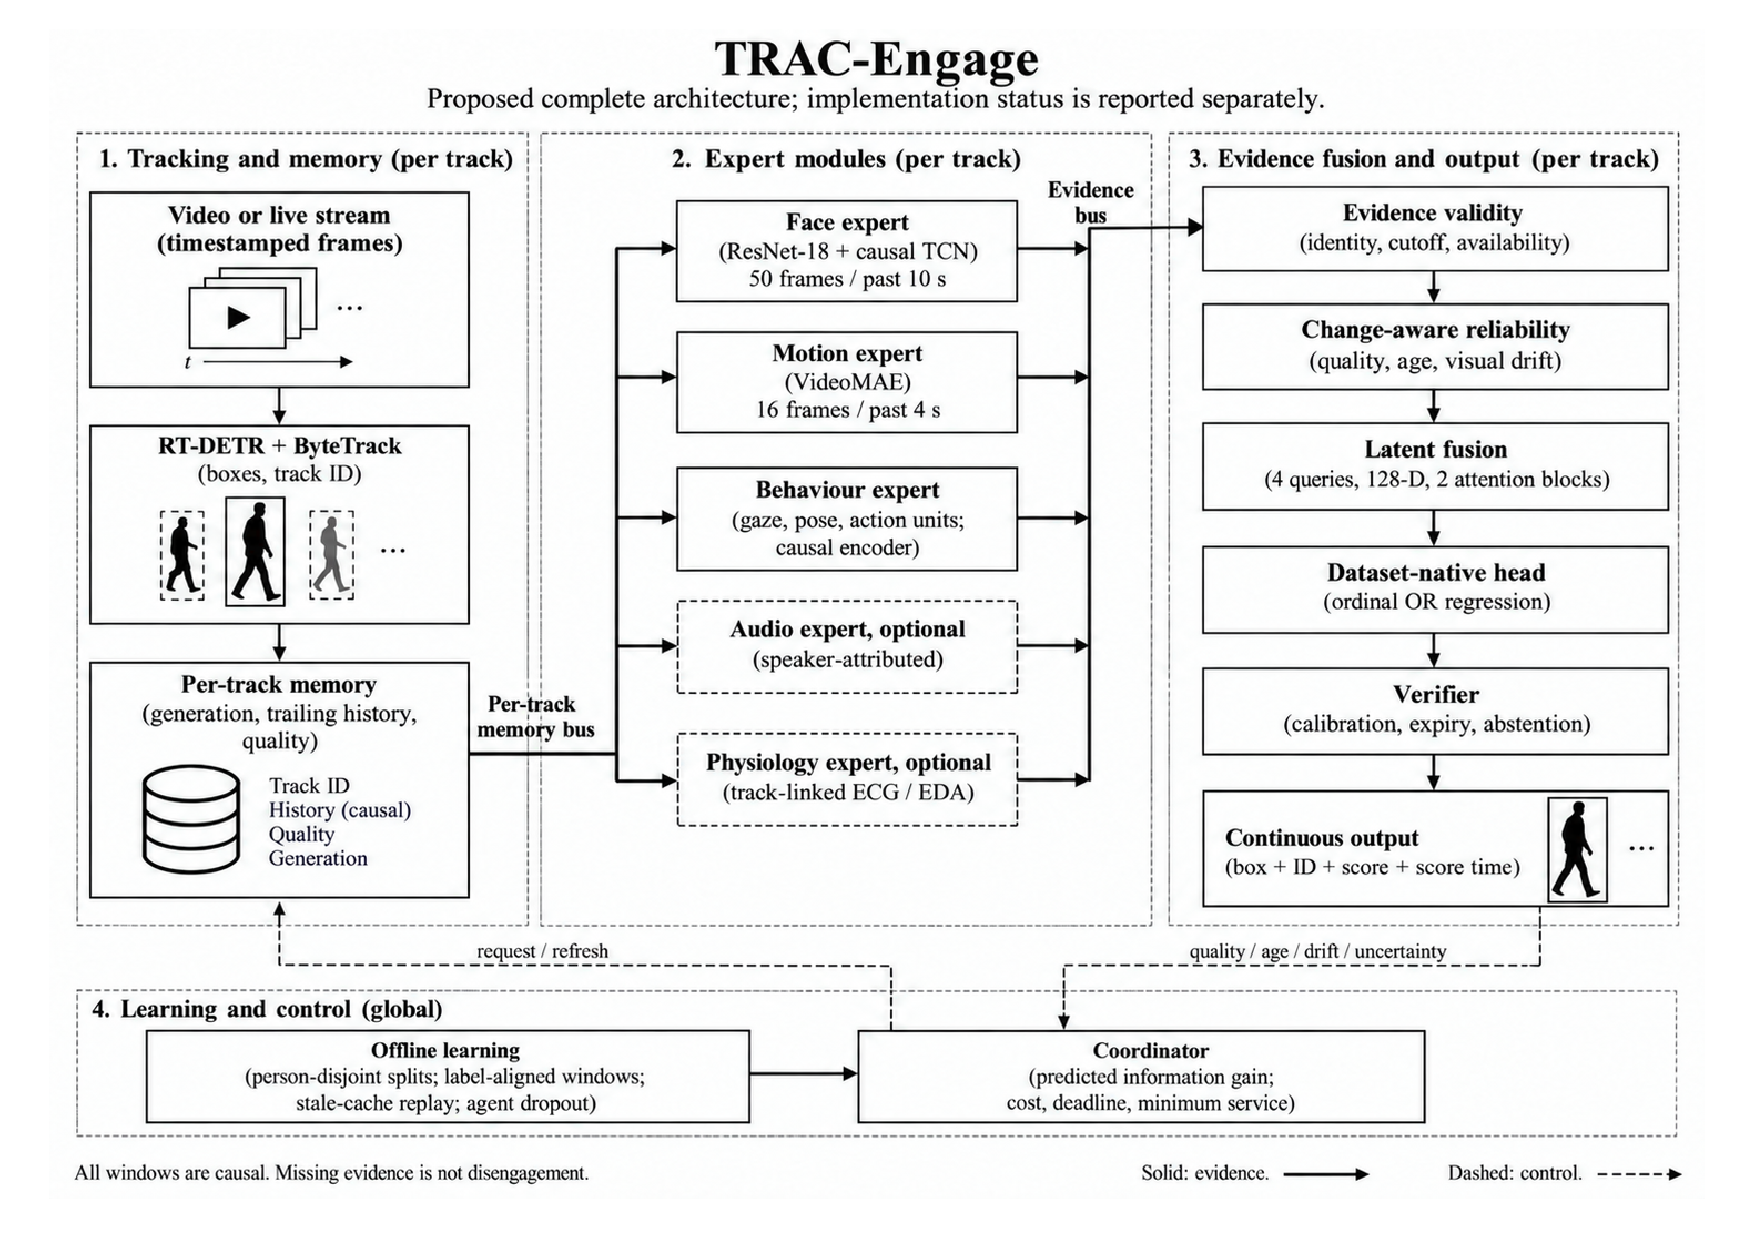
\includepdf[pages=1,fitpaper=true,pagecommand={}]{trac-engage-architecture-a4.pdf}
\end{document}
